\documentclass[10pt, conference, compsocconf]{IEEEtran}

\newif\ifnoTBD \noTBDfalse

% Uncomment to remove TBD macros
%\noTBDtrue

%\ifx\pdftexversion\undefined
%  \usepackage[dvips]{graphicx}
%\else
%  \usepackage[pdftex]{graphicx}
%  \usepackage{epstopdf}
%\fi

\ifnoTBD
\def\TBD#1{\typeout{TBD not done: #1}}
\else
\def\TBD#1{\textcolor{blue}{TBD: #1}}
\AtEndDocument{\typeout{ *** ATTENTION: compilation is in DRAFT
    mode. There might still be TBD that appear in the document ***}}
\fi

\usepackage[usenames]{color}
\usepackage{xspace}
\usepackage{listings}
%\usepackage{type1cm}
\usepackage{eso-pic}
\usepackage{subfigure}
\usepackage{multirow}
\usepackage{url}
\usepackage{latexsym}
%\usepackage{hyperref}
\usepackage{comment}
\usepackage{graphicx}

%\hypersetup{%
%  pdftitle={},
%  pdfauthor={George Bosilca},
%  pdfkeywords={network scheduling}
%  bookmarksnumbered, pdfstartview={FitH},
%  linkbordercolor={0 0 0},
%  citebordercolor={0 0 0},
%  urlbordercolor={0 0 0},
%  pdfborder={0 0 0},colorlinks={true},
%  linkcolor={0 0 0},
%  urlcolor=none,
%  citecolor=white
%}%

%\setlength{\oddsidemargin}{0in}   % origin is (1",1") from top-left corner
%\setlength{\evensidemargin}{0.0in}
%\setlength{\textwidth}{6.5in}
%\setlength{\textheight}{9in}
%\setlength{\topmargin}{0.0in}
%\setlength{\headheight}{0pt}
%\setlength{\headsep}{0pt}

\newcommand{\ompi}{Open\,MPI\xspace}
\newcommand{\ftla}{FT-LA\xspace}
\newcommand{\scalapack}{ScaLAPACK\xspace}
\newcommand{\abft}{Algorithmic Based Fault Tolerance\xspace}

\usepackage{algorithmic}
\usepackage{algorithm}
\usepackage{color}
\usepackage{amsthm}
\usepackage{amsfonts} 
\usepackage{amssymb,amsmath} 
\usepackage{graphicx}

\begin{document}

\title{Enabling Application Resilience With and Without the MPI Standard}
\author{
  \IEEEauthorblockN{Wesley Bland}
  \IEEEauthorblockA{Innovative Computing Laboratory, University of Tennessee, Knoxville\\
					wbland@eecs.utk.edu}\\
}

\maketitle

\begin{abstract}

As recent research has demonstrated, it is becoming a necessity for large scale
applications to have the ability to tolerate process failure during an
execution. As the number of processes increases, checkpoint/restart fault
tolerance approaches requiring large concurrent state checkpointing become untenable and radically new
methods to address fault tolerance are needed. This work addresses these
challenges by proposing a novel approach to a minimalistic fault discovery and
management model.  Such a model allows application to run to
completion despite fail-stop failures. As a proof of concept, in addition to the
proposed fault tolerance model, an implementation in the context of the \ompi
library is provided, evaluated and analyzed.
% as well as providing a corresponding implementation in the context of the
% \ompi project.  allow applications to discover and tolerate failures while
% continuing execution, all while minimizing application involvement. It
% includes modifications to the \ompi runtime as well as MPI library to give the
% user options when deciding how best to implement fault tolerance.

\end{abstract}


\begin{IEEEkeywords}
Fault Tolerance, Message Passing Interface, Distributed Runtime
\end{IEEEkeywords}

\section{Motivation} \label{sect:intro}

Fault tolerance is an increasingly necessary consideration in High Performance Computing (HPC). As machine sizes increase past hundreds of thousands of computing cores\footnote{http://www.top500.org} into the millions of computing resources, the likelihood of failures also increases. Observed failures rates are reaching between 1.8 and 3.6 failures per day on a system of only 635 nodes. This research confirms what has become an accepted reality of HPC going forward. Failures will occur at an increasing rate and for large scale applications to be useful, the failures will need to be handled in software while allowing the applications to continue running relatively uninterrupted.

This realization has lead to much research to attempt to solve the problems presented by the necessity for fault tolerance. The first and most well understood form of fault tolerance is rollback-recovery using periodic checkpointing. This form of fault tolerance has been widely adopted and works well for small scale machines where failure rates are expected to be relatively low. However, at larger scales, even with more reliable hardware, the  time spent performing checkpointing operations is expected to exceed the amount of time spent performing useful computation. To resolve this problem, we turn to Application Based Fault Tolerance (ABFT).

ABFT changes the way applications recover from failure. Rather than loading a previous checkpoint from disk and restarting an entire application, the algorithm itself recovers from the loss of a process and continues without the need to perform costly, large-scale checkpointing operations. The exact method used to recover from failures changes from application to application, but all applications have some requirements in common. The programming model and environment, together with the supporting runtime, need to provide basic functionality in order to allow applications to build a comprehensive fault management solution.

This is a challenging requirement. Most applications continue to use message passing to perform communication between processes, and in the message passing paradigm, collective communication is a popular and necessary way for groups of processes to communicate efficiently. However, collective communication also creates problems when trying to maintain the functionality of the communication library following a process failure due to the complex communication patterns and topologies that must be repaired. 

In addition to maintaining a functional communication library with scalable fault tolerance mechanisms, a fault tolerance solution must also provide extensibility. Because ABFT takes different forms for different applications, the fault tolerance provided by the communication library should also be able to adapt. For example, while one type of application may work best with a transactional model of fault tolerance where sections of the application are re-executed when recovery is necessary, a master-slave type of application may choose to simply spawn a replacement for any process which fails and continue on without needing further recovery.

To this end, we have modified a runtime system to support two new forms of fault tolerance within the message passing paradigm which can provide a suite of tools necessary for developers to include resilience in their applications. Due to size restrictions, details on the work implementing a resilient runtime can be found in~\cite{Bland:CCGrid12}.
%\section{Background \& Related Work}
\label{sect:background}

% Discuss some MPI-3 related proposals and issues

%Among the issues
%raised during the readings of the proposals, were the fact that these
%approaches will still incur a significant overhead on failure free
%operations, by requiring periodic \emph{consensus}

\subsection*{Background}

Message passing is the dominant form of communication used in parallel
applications, and MPI is the most popular library used to implement
it. However, as fault tolerance becomes a growing concern for
application developers, users have encountered some challenges with
the current MPI Standard that limit their options of fault tolerance
methods. The primary form of fault tolerance today is to periodically
write a checkpoint to disk.  While this method is effective in
allowing applications to recover from failures by restarting the work
from a previously saved point, it causes serious concerns on the
scalability~\cite{ExaScaleResilience09}. Moreover, such proactive
approach to fault tolerance requires a good idea of how many faults
might hurt the system, with which frequency and on what nodes. Many
works have discussed the optimal checkpointing period in the hope that
as few as possible of these preventive actions are taken by the
application~\cite{Young:1974, Gelenbe:1979, Plank01, Daly:2006,
  PreventiveCheckpointing11}. Unlike these works, the work presented
here focuses on {\it forward recovery}: checkpoint actions are taken
only {\emph after} a failure is detected, make it unnecessary to
hypothesize on an optimal checkpoint interval. The checkpoint interval
is optimal, by definition, as there will be one checkpoint interval by
effective fault.

An alternative approach to rollback recovery is to take advantage of
the properties of the application to design it as naturally fault-tolerant. This
technique is traditionally called \abft \cite{huang1984algorithm}. The
algorithm itself includes modifications, or additional steps, to cope
with the loss of some of its data. It includes a modification of the
algorithm, usually to maintain redundant information in the data
during the life of the application, and a recovery procedure that
works only with the data remaining after the failure is detected, and
reconstructs the missing data using additional computation and
communication. To support such an algorithm, the underlying
programming environment must however provide a way to communicate
after the failure occurs on one of the processes.

The current MPI Standard (MPI-2.2,~\cite{MPI22}) does not provide
significant help to deal with that type of behavior. Section~2.8
states in the first paragraph: ``\emph{MPI does not provide mechanisms
  for dealing with failures in the communication system. [...]
  Whenever possible, such failures will be reflected as errors in the
  relevant communication call. Similarly, MPI itself provides no
  mechanisms for handling processor failures.}'' Failures, be they due
to a broken link or a dead process are considered as resource
errors. Later, in the same section: ``\emph{This document does not
  specify the state of a computation after an erroneous MPI call has
  occurred. The desired behavior is that a relevant error code be
  returned, and the effect of the error be localized to the greatest
  possible extent.}'' So, for the current standard, process or
communication failures are to be handled as errors, and the behavior
of the MPI application after an error has been returned is left
unspecified by the standard. However, the standard does not prevent
implementations to go beyond its requirements, and on the contrary,
encourages high-quality implementations \emph{to return} errors once a
failure is detected.

Unfortunately, most of the implementations of the MPI Standard have
taken the path of considering process failures as unrecoverable
errors, and the processes of the application are most often killed by
the runtime system, when a failure hits any of them. The runtime
system then returns with an error code, signaling the failure of the
run, leaving no other choice to the user but to run a new parallel
execution.

The MPI forum is currently examining options for the future direction
of MPI for MPI-3. One of the workgroups is dedicated to propose a
standard form of MPI-supported fault tolerance. The proposal outlines
a method of run-through stabilization which allows the application to
acknowledge and repair communications, both collectively and between
specific ranks in a point-to-point way~\cite{Hursey11MPI3FT}. The
emphasis of the proposal is a set of "validation" functions which the
application is required to call to repair and re-enable communication within
an MPI communicator containing a failed process. To repair point to
point wildcard receives, the application needs to collectively call the function
MPI\_COMM\_REENABLE\_ANY\_SOURCE. To repair collective communication
within a communicator, the application needs to call the function
MPI\_COMM\_VALIDATE.  These functions give the MPI implementation an
opportunity to acknowledge failures and discover or ensure that other
MPI processes also acknowledge the same failures. It also gives the
MPI library a chance to repair communication channels between
remaining processes, optimizing communication topologies if possible
and necessary.

While this method of fault tolerance is sufficient for \abft, it is
not without its drawbacks. The calls necessary to recover from
collectives incur a non-trivial overhead even during the fault free
case. MPI\_COMM\_VALIDATE requires a distributed consensus algorithm
which is currently best implemented at log
scale~\cite{Hursey11LogConsensus}. While this level of overhead is
better than the current state of the art of periodic checkpointing, it
still presents a significant cost that not all applications want or
need to pay to check the validity of the communicators. Most
importantly, this proposal does not yet include process recovery,
which is left to a future proposal to the MPI forum.

% Discuss issues in general with FT-MPI like approaches, besides the 
% sheer problem of standard adoption

% Explain why it is not believed that ABFT can perform without REPLACE 
% or BLANK, or leave it for next section ?

\subsection*{Related Work}

FT-MPI~\cite{fagg2000ft} is an MPI-1 implementation which added
extensions to the MPI standard to give users options for their
\abft. FT-MPI proposed to change the MPI semantics of some of the
calls, to enable continuing the execution of the parallel application
after a failure hits the system, and to rebuild the communicators, thus
re-enabling communications. This approach has been proven successful,
and some applications have been implemented relying on the features of
FT-MPI. However, these modifications of the standard were not imported
in the official MPI standard, and no other MPI implementation took the
same approach. The lack of large distribution of the FT-MPI
implementation prevented a large base of users from implementing their
solution based on this proposition.

%  One of
% the solutions implemented in FT-MPI was to introduce a new MPI\_Errhandler
% called MPI\_ERRORS\_BLANK. This MPI\_Errhandler replaced the position of the
% failed processes inside a communicator with MPI\_PROC\_NULL. By using this
% semantic, the remaining MPI calls could function normally as communication with
% MPI\_PROC\_NULL always succeeds. When FT-MPI encountered a fault, it destroyed
% all MPI Communicators and required that the application recreate them to account
% for the failed processes. While this was a useful step in allowing the most
% level of flexibility from the application's perspective, it made recovery very
% complex and added a large overhead.

% FT-MPI is another form of fault tolerance that can be successful for some, but in
% applications that require that all processes be running to reach successful
% completion, having a hole in the communicator is not a valid solution. The
% failed processes need to somehow be recovered.

%\TBD{Anything needed from the QR side of things?}

Besides the works that have been cited previously to present the
problem statement, the different approaches that have been proposed,
and how this approach is original, the article by W. Gropp and E. Lusk
in 2004 \cite{Gropp:2004:FTM:1080704.1080714} is the work closest to
the On-Demand Checkpointing, from the MPI requirement perspective.  In
this article, the authors explain how the standard can be interpreted,
or slightly modified, to allow for a form of fault tolerance. They
consider different approaches: periodical checkpointing; using
inter-communicators and separate MPI applications to contain an error
in an MPI application; modifying the MPI semantics; or propose new
extensions. However, the last three propositions demand more from the
MPI implementation than we require in this work: for example, the MPI
library is supposed to continue its normal execution, if the error was
located in another MPI application, connected with the one subject to
the error through an inter-communicator. In our work we do not even
require such a step: the only
demand on the MPI implementation is that it does not forcibly kill the
living processes without letting them take a checkpoint, but returns
an error. Once this is ensured, no requirement from any MPI call is
needed.

Moreover, we illustrate the well soundness of our approach using a
non-trivial algorithm: a QR factorization, that is made fault tolerant
using the modified \ompi, and the On-Demand Checkpointing
technique. We demonstrate that this approach is functional, and
evaluate its performance at large scale.

\section{Related Work}
\label{sect:related}

Efforts toward fault tolerance in MPI have previously been attempted.  Automatic
fault tolerance~\cite{Bouteiller10Redesign,MPICHVblocking} is a compelling
approach for users, as failures are completely masked and handled internally by
the MPI library, which requires no new interfaces to MPI or application code
changes. Unfortunately, many recent studies point out that automatic approaches,
either based on checkpoints or replication, will exhibit poor efficiency on
Exaflop platforms~\cite{BOSILCA-2012-696154,lawn265}.

Application Based Fault Tolerance
(ABFT)~\cite{fthpl2011,pengduppopp12,huang1984algorithm} is another approach
that promises better scalability, at the cost of significant algorithm and 
application code changes. Despite some limited 
successes~\cite{europar12/onfailureckpt,Gropp:2004:FTM:1080704.1080714},
MPI interfaces need to be extended to effectively support ABFT. The most notable past 
effort is FT-MPI~\cite{fagg2000ft}, which provided several recovery modes for the user 
but was never standardized and therefore was not portable enough for most users.
\section{Runtime} \label{sect:runtime}

We present in this section how the \ompi Runtime Environment
(ORTE)~\cite{Castain:2008dx} has been modified to become resilient as an example
of the expected changes that need to be undergone on other runtime environments
to provide resilient capabilities. We focus first on how the runtime itself has
been made fault tolerant; then on the additional services that the runtime
should provide to the MPI library or any other fault-aware parallel environment:
Failure Detection and Notification. 
% The modified runtime is capable of running any MPI application.
%However, since the MPI level does not provide a
%stabilization interface yet, the MPI application cannot use the additional
%services to continue its execution.

\subsection{Out-Of-Band Message Consistency Using Epochs} \label{subsect:epochs}

Before implementing process recovery, a way of tracking the status of processes
is necessary. A commonly used method in literature is to add an epoch to the
process naming scheme. By incrementing the epoch every time the {\em Head Node
Process} (HNP) is notified of a failure, we can use it to track the number of
times an individual process has failed.  The runtime uses this epoch to prevent
transient process failures from introducing unexpected behavior by cutting off a
process with an epoch less than the most recent value from interfering with the
other processes.  As each message is processed by the communication library, it
is checked against the most recent known epoch for the originating process. If
the message's epoch is less than the most recently known epoch, the message is
dropped and will need to be retransmitted to the new version of the previously
failed process. This essentially imposes a fail-stop fault model~\cite{FLP85}
upon the processes, simplifying error detection and recovery.
	
\subsection{Fault Handling} \label{subsect:failure_handling}

Concurrently with the notification of failure throughout the runtime, the HNP
and the ORTE daemons (ORTEDs) also perform fault handling tasks to stabilize the
runtime and allow processes to continue. The most noticeable portion of the
runtime that must be updated is the routing layer. Most routing layers have some
sort of underlying topology that passes messages from one node to the next rather than all
messages being routed through a central entity, or allowing direct communication
between nodes for the out-of-band messaging system. The latter would require
$n^2$ opened connections, imposing a huge load on the system. This routing layer
must be mended after any of the nodes fail. One of the most common routing
topologies is a tree. When the fault is detected, the tree must remove the
faulty process and create connections from the failed process's parent to its
children. This must also take into account any subsequent failures so that if
necessary, the routing layer will continue to look upward or downward in the
tree to find the closest living neighbor and prevent any child from becoming
orphan due to a lack of connection to a living parent.
%  Another option would be
% to completely rebuild the tree after each failure. This method introduces other
% complications such as handling in-flight messages or active collective and this
% is left for a possible future improvement.

\subsection{Failure Detection} \label{subsect:failure_detection}

Failure detection is accomplished using the existing detectors in ORTE. The
primary detection method is to monitor the status of communication channels. If
a connection fails, the ORTE error handler begins the process of managing the
fault as detailed in Section~\ref{subsect:failure_handling}. In the future, when
an MPI layer will be placed on top of the runtime, it will need to send errors
to the runtime to allow errors to be handled in a consistent way. The current
method of handling failures in \ompi is to abort as soon as possible after
detecting an error. By passing the error information to the runtime rather than
acting within the MPI layer, that singular method of handling faults can be
improved and the application may survive the fault.

\subsection{Failure Notification} \label{subsect:failure_notification}

When a failure occurs, ORTE quickly attempts to stabilize the runtime system to
allow the surviving processes to continue. The first step in this process is to
notify the HNP. The HNP is responsible for maintaining the state of the
application and notifying all runtime processes of any changes to which they
need to respond. Once the HNP has received the message from the ORTEDs who
detected the failure, it broadcasts this information to all other daemons.
While some of them might already know about the failure, because they detected
it via the direct connections between daemons, by including the epoch of the
failed process they can prevent duplicate or out-of-order handling of the
faults. At this point, the runtime would notify the MPI layer of the error,
therefore allowing the MPI processes themselves to decide how the parallel
application will react to the fault.


\section{MPI} \label{sect:mpi}

% What does the current standard do?

The current MPI standard does not provide much guidance for applications in
presence of faults. According to the standard, when implementing a high-quality
MPI library, the application should regain control following a process failure.
This control gives the application the opportunity to save its state and exit
gracefully, rather than the usual behavior of being aborted by the MPI
implementation itself. This makes continuing meaningful execution very difficult
and usually requires the application to restart itself from a previously saved checkpoint.

% What kind of FT can we do with it?

% One opportunity to use the current MPI standard without modification is to use
% the MPI error handler MPI\_ERRORS\_RETURN rather than MPI\_ERRORS\_ABORT. This
% would allow the application to write a checkpoint which it can use to restart
% itself from the current point with a clean MPI library. However, this requires
% an application that is already fault tolerant and can continue without the failed
% process or can recreate the lost data from the failed process. While this class
% of Application Based Fault Tolerant algorithms does exist, it does not encompass
% the vast majority of applications.

% What departures did we create from the standard?

Our work deviates from the current standard to provide a more flexible suite
of tools to implement fault tolerance. 
%
If a process failed during an MPI call, the call will return an error code to
reflect the failure. This allows the application to know that a process has
failed and to perform any internal recovery operations necessary. Once the
application has been alerted via the MPI return code, the application will not
receive another notification until a new process fails. By not requiring an
acknowledgment from the remaining processes, our method of fault tolerance
imposes as little burden on the applications as possible and allows failure free
executions to incur the minimum amount of overhead.

As most of the MPI applications take advantage, in addition from point-to-point
message, of collective communications, we took a particular interest in
providing a clear semantic of how fault can integrate with collective
communications. We are implementing fault
tolerant collective operations which allow the application to run collectives
over MPI\_Communicators including failed processes. For collectives which do not
include any data, such as MPI\_Barrier, this is simple enough operation.  For
collectives which require data combination, such as MPI\_Gather or MPI\_Reduce,
this can be a slightly more complicated task. However, all of the MPI collective
operations can eventually be simplified to a communicator pattern with some
amount of data, which may or may not be combined with or without an operation in
the process. When determining how many processes to include in the collective
operation, our MPI library does not include the failed processes. Also, when a
process fails during a collective, the operation is updated to remove the failed
process. Once the participating group is determined, we can continue the MPI
collective as if no failures occurred.

This work will also eventually include process recovery which will allow the
application to decide to recreate the failed process by launching a new MPI rank
on a fault free node. The user will be responsible for bringing the new rank
back to the point of the failure, but this will support another set of
applications which require a specific number of processes to continue in the
presence of a process failure.  The specifics of the process recovery techniques
are not yet ready for publication.

\section{Performance Discussion}\label{sec:experiments}

In this section, we use our \ompi and \abft QR implementations to
evaluate the performance of the \cof protocol. We
use two test platforms. The first machine, ``Dancer,'' is a 16-node
cluster. All nodes are equipped with two 2.27GHz quad-core Intel E5520
CPUs, with a 20GB/s Infiniband interconnect. Solid State Drive disks are
used as the checkpoint storage media. The second system is the Kraken
supercomputer. Kraken is a Cray XT5 machine, with 9,408 compute nodes.
Each node has two Istanbul 2.6 GHz six-core AMD Opteron processors, 16
GB of memory, and are connected through the SeaStar2+ interconnect. The
scalable cluster file system ``Lustre'' is used to store checkpoints.

\subsection{MPI Library Overhead}

One of the concerns with fault tolerance is the amount of overhead
introduced by the fault tolerance management additions. Our
implementation of fault detection and notification is mostly implemented
in the non-critical ORTE runtime. Typical HPC systems
feature a separated service network (usually Ethernet based) and a
performance interconnect, hence health monitoring traffic, which happens
on the OOB service network, is physically separated from the MPI
communications, leaving no opportunity for network jitter. Changes to
MPI functions are minimal: the same condition that used to trigger
unconditional abort has been repurposed to trigger error handlers. As
expected, no impact on MPI bandwidth or latency was measured
(Infiniband and Portals results not shown for lack of space). The memory
usage of the MPI library is slightly increased, as the incarnation
number doubles the size of process names; however, this is negligible in
typical deployments.

\subsection{Failure Detection}

According to the requirement specified in Section~\ref{sec:interface}, only
in-band failure detection is required to enable \cof. Processes detecting a
failure checkpoint then exit, cascading the failure to processes communicating
with them. However, no recovery action (in particular checkpointing) can take 
place before a failure has been
notified. Thanks to asynchronous failure propagation in the
runtime, responsiveness can be greatly improved, with a high probability for the
next MPI call to detect the failures, regardless of communication pattern or
checkpoint duration.

\begin{figure}[htb]
\centering 
  \subfigure[Linear OOB Routing]{
    \label{fig:linear}
    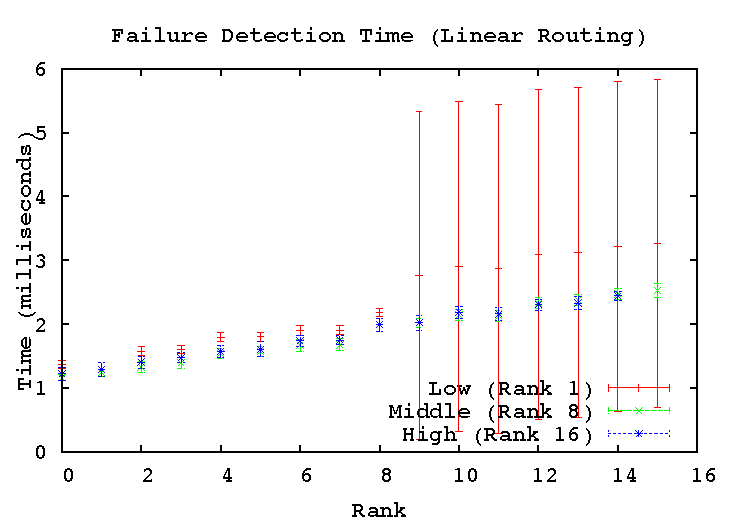
\includegraphics[width=.43\linewidth]{figures/failure_detection_linear_errbars}}
  \hfill
  \subfigure[Binomial OOB Routing]{
    \label{fig:binomial}
    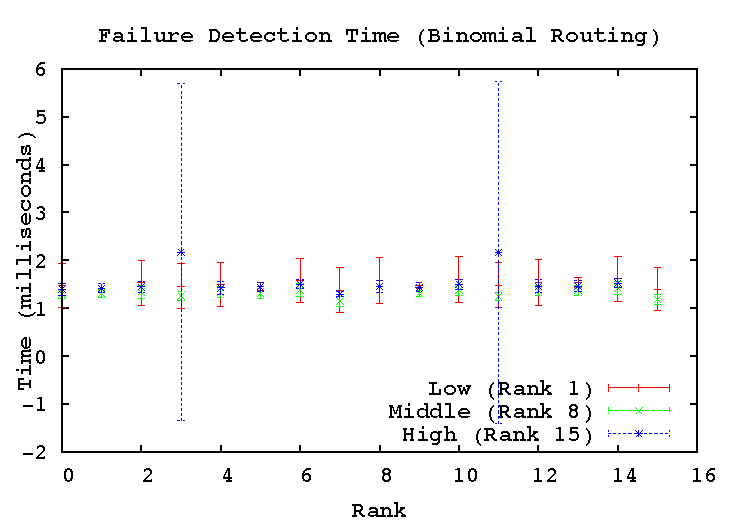
\includegraphics[width=.43\linewidth]{figures/failure_detection_binomial_errbars}}\vspace{-.2cm}
\caption{Failure detection time, sorted by process rank, depending on the OOB overlay network used for 
failure propagation.}\label{fig:detect}
\end{figure}

We designed a micro-benchmark to measure failure detection time as
experienced by MPI processes. The benchmark code synchronizes with an
MPI\_Barrier, stores the reference date, injects a failure at a specific
rank, and enters a ring algorithm until the MPI error handler stores the
detection date. The OOB routing topology used by the ORTE runtime introduces a
non-uniform distance to the failed process, hence failure detection time
experienced by a process may vary with the position of the failed
process in the topology, and the OOB topology. Figure~\ref{fig:linear}
and~\ref{fig:binomial} present the case of the linear and
binomial OOB topologies, respectively. The curves ``Low, Middle, High'' present the
behavior for failures happening at different positions in the OOB
topology. On the horizontal axis is the rank of the detecting process,
on the vertical axis is the detection time it experienced. The
experiment uses 16 nodes, with one process per node, MPI over Infiniband, OOB
over Ethernet, an average of 20 runs, and the MPI barrier latency is four orders of
magnitude lower than measured values.

In the linear topology (Figure~\ref{fig:linear}) every runtime process
is connected to the \emph{mpirun} process. For a higher rank, failure
detection time increases linearly because it is notified by the
\emph{mpirun} process only after the notification has been sent to all
lower ranks. This issue is bound to increase with scale. The binomial
tree topology (Figure~\ref{fig:binomial}) exhibits a similar best
failure detection time. However, this more scalable topology has a low
output degree and eliminates most contentions on outgoing messages,
resulting in a more stable, lower average detection time, regardless of the
failure position. Overall, failure detection time is on the order of
milliseconds, a much smaller figure than typical checkpoint time.

% WE SHOULD HAVE SOME RESULTS WITH AUTO-FT AND/OR APP BASED PERIODIC CHECKPOINT



\begin{figure}[thb]
\centering
\begin{minipage}[t]{.29\linewidth}
	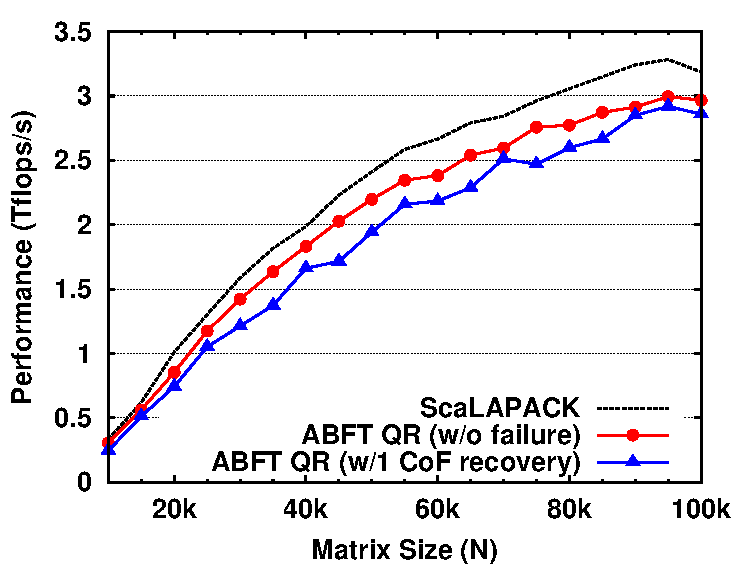
\includegraphics[width=\linewidth]{figures/kraken_new_data}
	\vspace{-.6cm}\caption{ABFT QR and one \cof recovery on Kraken (Lustre).}%($24\times 24$ grid)
	\label{fig:kraken_performance}	
\end{minipage}
\hfill
\begin{minipage}[t]{.29\linewidth}
    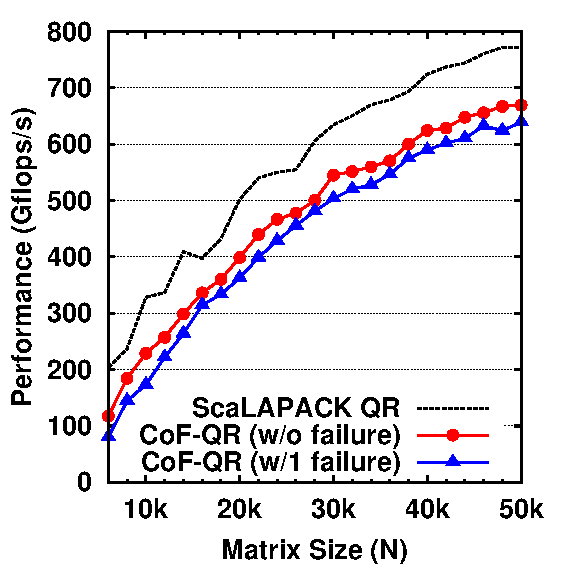
\includegraphics[width=\linewidth]{figures/dancer_performance_data}
	\vspace{-.6cm}\caption{ABFT QR and one \cof recovery on Dancer (local SSD).} %($16\times 8$ grid)
    \label{fig:dancer_performance}
\end{minipage}
\hfill
\begin{minipage}[t]{.29\linewidth}
    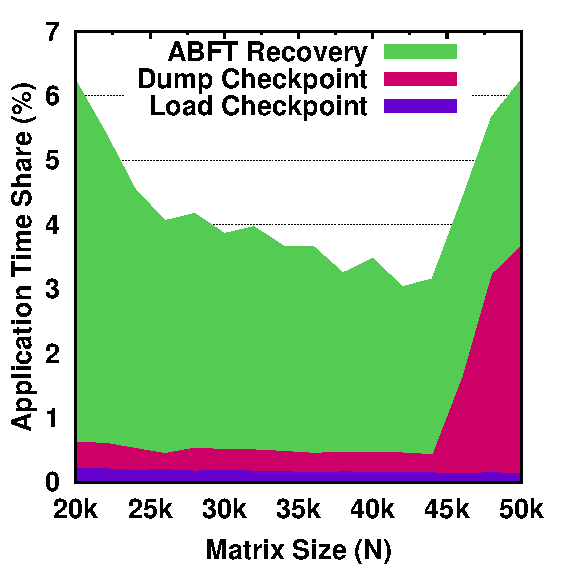
\includegraphics[width=\linewidth]{figures/dancer_1_error_timing_process_new_data}
	\vspace{-.6cm}\caption{Time breakdown of one \cof recovery on Dancer (local SSD).}
    \label{fig:dancer_timing}
\end{minipage}\vspace{-.3cm}
\end{figure}

\subsection{Checkpoint-on-Failure QR Performance}

\paragraph*{Supercomputer Performance:}
Figure~\ref{fig:kraken_performance} presents the performance on the
Kraken supercomputer. The process grid is $24\times 24$ and the block size
is 100. The \cof-QR (no failure) presents the performance of the \cof QR
implementation, in a fault-free execution; it is noteworthy, that when
there are no failures, the performance is exactly identical to the
performance of the unmodified FT-QR implementation. The \cof-QR (with
failure) curves present the performance when a failure is injected after
the first step of the PDLARFB kernel. The performance of the non-fault
tolerant ScaLAPACK QR is also presented for reference.

Without failures, the performance overhead compared to the regular
ScaLAPACK is caused by the extra computation to maintain the checksums inherent to the \abft
algorithm~\cite{pengduppopp12}; this extra computation is unchanged between \cof-QR and
FT-QR. Only on runs where a failure happened do the \cof protocols
undergoe the supplementary overhead of storing and reloading
checkpoints. However, the performance of the \cof-QR remains very
close to the no-failure case. For instance, at matrix size N=100,000,
\cof-QR still achieves 2.86 Tflop/s after recovering from a failure,
which is 90\% of the performance of the non-fault tolerant ScaLAPACK QR.
This demonstrates that the \cof protocol enables efficient, practical
recovery schemes on supercomputers.

\paragraph*{Impact of Local Checkpoint Storage:}

Figure~\ref{fig:dancer_performance} presents the performance of the \cof-QR 
implementation on the Dancer cluster with a $8\times 16$ process
grid. Although a smaller test platform, the Dancer cluster features
local storage on nodes and a variety of performance analysis tools
unavailable on Kraken. As expected (see~\cite{pengduppopp12}), the \abft
method has a higher relative cost on this smaller machine. Compared to
the Kraken platform, the relative cost of \cof failure recovery is
smaller on Dancer. The \cof protocol incurs disk accesses to store and
load checkpoints when a failure hits, hence the recovery overhead
depends on I/O performance. By breaking down the relative cost of each
recovery step in \cof, Figure~\ref{fig:dancer_timing} shows that
checkpoint saving and loading only take a small percentage of the total
run-time, thanks to the availability of solid state disks on every node.
Since checkpoint reloading immediately follows checkpointing, the OS
cache satisfy most disk access, resulting in high I/O performance. For
matrices larger than N=44,000, the memory usage on each node is high and
decrease the available space for disk cache, explaining the decline in
I/O performance and the higher cost of checkpoint management. Overall,
the presence of fast local storage can be leveraged by the \cof protocol
to speedup recovery (unlike periodic checkpointing, which
depends on remote storage by construction). Nonetheless, as demonstrated by the
efficiency on Kraken, while this is a valuable optimization, it is not a
mandatory requirement for satisfactory performance.

%On a problem of this size, the additional overheads
%are dominated by the time it takes to terminate the failing MPI
%application and relaunch a new one. 

\section{Conclusion}
\label{sect:conclusion}

Many responsible voices agree that sharp increases in the volatility of future,
extreme scale computing platforms are likely to imperil our ability to use them
for advanced applications that deliver meaningful scientific results and
maximize research productivity. Since MPI is currently, and will likely continue
to be -- in the medium-term -- both the de-facto programming model for
distributed applications and the default execution model for large scale
platforms running at the bleeding edge, it is the place in the software
infrastructure where semantic and run-time support for application faults needs
to be provided.

The \ulfm proposal is a careful but important step forward toward accomplishing
this goal delivering support for a number of new and innovative resilience
techniques through simple, familiar API calls, but it is backward compatible
with previous versions of the MPI standard, so that non fault-tolerant
applications (legacy or otherwise) are supported without any changes to the
code. Perhaps most significantly, applications can use \ulfm-enabled MPI without
experiencing any degradation in their performance, as we demonstrate in this
paper. Some of these applications along with other portable libraries are
currently being refactored to take advantage of \ulfm semantics.

The author would like to acknowledge his co-authors in the full
paper~\cite{Bland:2012tp}: Aurelien Bouteiller, Thomas Herault, Joshua Hursey,
George Bosilca, and Jack J. Dongarra.


\newcommand{\BIBdecl}{\setlength{\itemsep}{0.03\baselineskip}} 
\bibliographystyle{IEEEtran}
\bibliography{resil-mpi-ccgrid}

\end{document}

